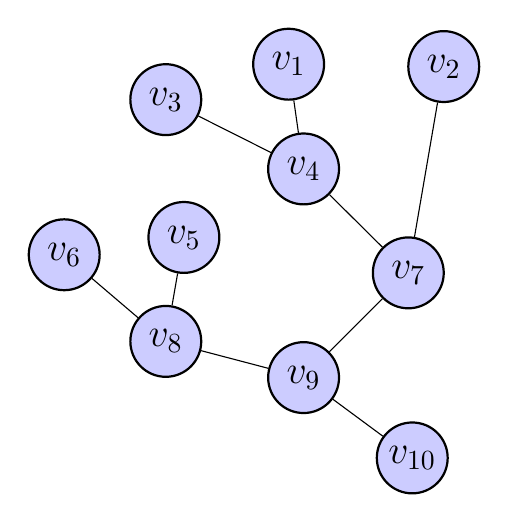
\begin{tikzpicture}[
  scale=1,
  vnode/.style={circle, fill=blue!20, draw=black, thick, minimum size=9mm, inner sep=0pt, font=\Large}
]
  % Vértices
  \node[vnode] (v1) at (3.73, 5.25) {$v_1$};
  \node[vnode] (v2) at (5.70, 5.22) {$v_2$};
  \node[vnode] (v3) at (2.17, 4.80) {$v_3$};
  \node[vnode] (v4) at (3.92, 3.92) {$v_4$};
  \node[vnode] (v5) at (2.40, 3.05) {$v_5$};
  \node[vnode] (v6) at (0.88, 2.83) {$v_6$};
  \node[vnode] (v7) at (5.25, 2.60) {$v_7$};
  \node[vnode] (v8) at (2.17, 1.73) {$v_8$};
  \node[vnode] (v9) at (3.92, 1.27) {$v_9$};
  \node[vnode] (v10) at (5.30, 0.25) {$v_{10}$};

  % Aristas
  \foreach \from/\to in {v1/v4, v2/v7, v3/v4, v4/v7, v5/v8, v6/v8, v7/v9, v8/v9, v9/v10}
    \draw (\from) -- (\to);
\end{tikzpicture}
